\documentclass[tikz,border=2mm]{standalone}

\begin{document}
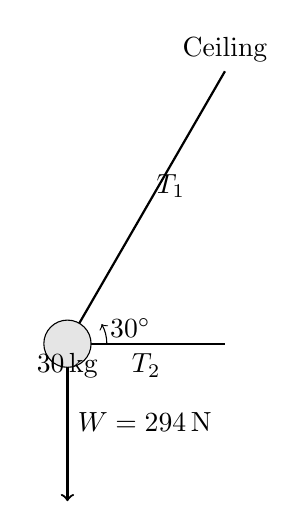
\begin{tikzpicture}

% Define coordinates
\coordinate (O) at (0,0); % Origin (mass location)
\coordinate (A) at (2,3.46); % End of inclined cord
\coordinate (B) at (2,0); % End of horizontal cord

% Draw cords
\draw[thick] (O) -- (A) node[midway, above right] {$T_1$};
\draw[thick] (O) -- (B) node[midway, below] {$T_2$};

% Draw weight
\draw[thick, ->] (O) -- ++(0,-2) node[midway, right] {$W = 294\, \mathrm{N}$};

% Draw angles
\draw[->] (0.5,0) arc[start angle=0, end angle=30, radius=0.5];
\node at (0.8,0.2) {$30^\circ$};

% Draw mass
\filldraw[fill=gray!20] (O) circle (3mm) node[below] {$30\, \mathrm{kg}$};

% Add labels for key points
\node[above] at (A) {Ceiling};

\end{tikzpicture}
\end{document}
